\documentclass[12pt,tikz,border=8pt]{standalone}
\usepackage{libertine}
\usepackage{amsmath,amssymb}
\usepackage{tikz}
\usetikzlibrary{arrows.meta}

\begin{document}
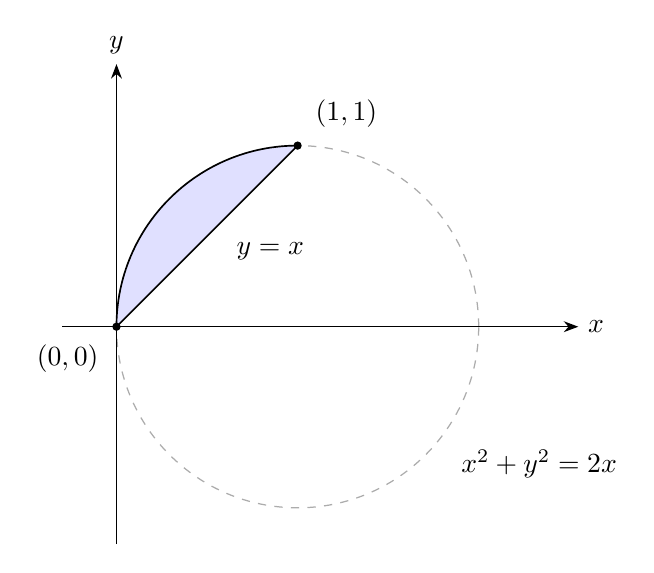
\begin{tikzpicture}[x=2.3cm,y=2.3cm,>=Stealth,
  boundary/.style={black,line width=0.6pt},
  every node/.style={font=\normalsize}]
  % The region is inside the shifted disk and above y=x.
  % Its curved boundary follows the circle from angle 180 to angle 90.
  \fill[blue!12] (0,0)
    arc[start angle=180,end angle=90,radius=1] -- cycle;

  \draw[gray!65,line width=0.45pt,dashed] (1,0) circle[radius=1];
  \draw[->,line width=0.5pt] (-0.3,0) -- (2.55,0)
    node[right] {$x$};
  \draw[->,line width=0.5pt] (0,-1.2) -- (0,1.45)
    node[above] {$y$};

  \draw[boundary] (0,0)
    arc[start angle=180,end angle=90,radius=1] -- cycle;

  \fill (0,0) circle[radius=1.5pt]
    node[below left=3pt] {$(0,0)$};
  \fill (1,1) circle[radius=1.5pt]
    node[above right=3pt] {$(1,1)$};

  \node[below right] at (0.61,0.52) {$y=x$};
  \node[right] at (1.85,-0.76) {$x^2+y^2=2x$};
\end{tikzpicture}
\end{document}
